\subsection{User Interface Level}

Dr.~Miguel Canals and Andre Amador have stated that the system currently being used, although functional, has a series of problems that limit their experiments.  These limitations include not being able to let the sphere run free due to the lack of a location system, the need of breaking the sphere to include a button to turn it on, the need to open the sphere in order to get the data, the need to wait until the spheres are completely dry in order to be able to open them to prevent hardware damage, the inability to take out the data in the field, the inability to do these experiments at night due to the fear of losing sight of them and the inability to reuse the sphere right away for another experiment (because of the way the data is collected) 

In order to attend their needs, the proposed system will be divided in two parts from the user's perspective: the sphere and a computer interface. The sphere will contain an LED that will be turned on during the night to help the user find the sphere, allowing them to do their work at night.  The LED will also serve to indicate transfer and battery status.  

On the computer, the user will have a simple program with a Graphical User Interface (GUI) that will enable them to interact with the spheres. Figure~\ref{fig:gui} shows a mock-up illustrating the concept of how the GUI might look like but does not aim to depict the final product.  As it can be seen, the proposed GUI displays options for locating spheres, turning the sphere system ON or OFF, changing the sample interval, retrieving data from an individual sphere or from all at the same time, deleting the data from one sphere or from all of them, manually turning on the LED strobe and seeing additional information for each sphere such as ID number, sample start date and last retrieved location. Features and options, as well as the look, will change on the final product based on the necessities and requirements of the researchers, which are, ultimately, the end-users.

\begin{figure}[H]
	\centering
	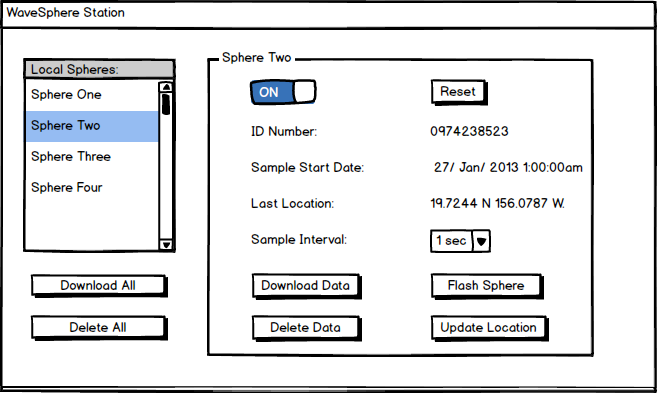
\includegraphics[scale=0.6]{img/gui.png}
	\caption{Graphical User Interface of the software housed in the computer acting as a base station. \label{fig:gui}}
\end{figure}
